\chapter{Benchmark Specification}
\label{sec:benchmark-specification}

\paragraph{Overview}
The LDBC Social Network Benchmark workloads require several components to generate data and updates, produce query substitution parameters, run the benchmark on the system under test, \etc
\autoref{fig:snb-overview} shows a blueprint for the frameworks implementing the \ldbcsnb benchmark workloads.

\begin{figure}[htbp]
    \centering
    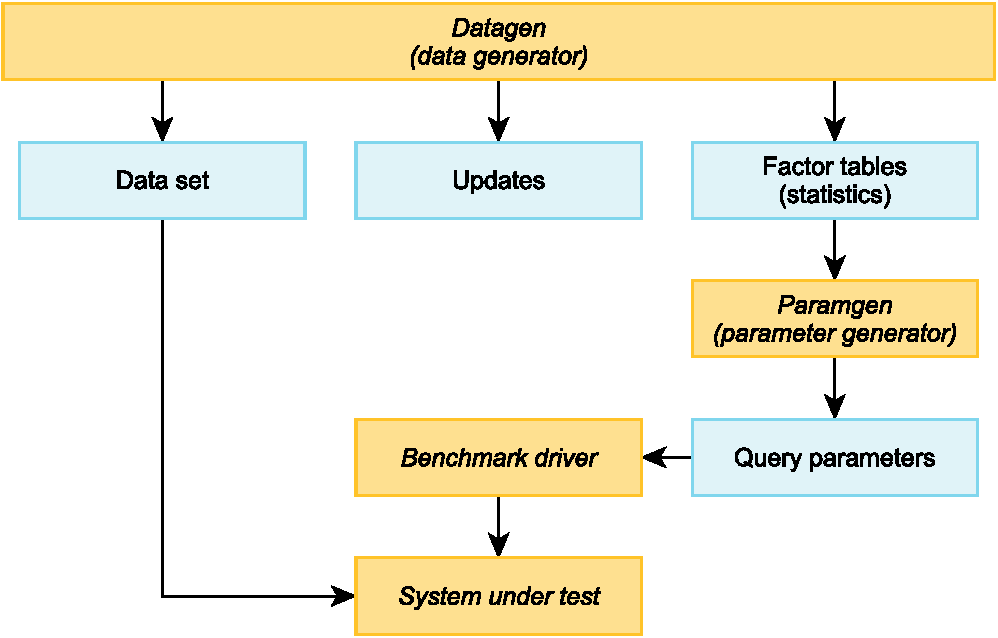
\includegraphics[scale=\yedscale]{figures/snb-overview}
    \caption{
        High-level overview of the frameworks implementing each LDBC Social Network Benchmark workload.
        Legend:
        \fcolorbox{mydarkyellow}{mylightyellow}{{\scriptsize \textit{\textsf{Software component}}}}
        \fcolorbox{mydarkblue}{mylightblue}{{\scriptsize \textsf{Data artifact\vphantom{p}}}}
    }
    \label{fig:snb-overview}
\end{figure}

\paragraph*{Portability}
\ldbcsnb is designed to be flexible and to have an affordable entry point. \ldbcsnb aims to accommodate systems from single node in-memory systems to large distributed multi-node clusters. Therefore, the requirements to fulfill for executing \ldbcsnb are limited to pure software requirements to be able to run the tools.
While the benchmark specification aims to be portable, the software provided by \ldbcsnb have been primarily tested on Linux-based operating systems (\eg Ubuntu LTS). The driver and clients for the reference implementations were implemented in Java. The generator has two versions: the Hadoop-based one was written in Java, while the Spark-based one is written in a mix of Java and Scala. 

\paragraph*{Auditable systems}
\ldbcsnb does not impose the usage of any specific type of system, as it targets systems of different nature and characteristics, from graph databases, graph processing frameworks and RDF systems, to traditional relational database management systems. Therefore, data can be stored in the most convenient manner the test sponsor may decide, as long as it conforms with the execution rules.
